% Options for packages loaded elsewhere
\PassOptionsToPackage{unicode}{hyperref}
\PassOptionsToPackage{hyphens}{url}
\PassOptionsToPackage{dvipsnames,svgnames*,x11names*}{xcolor}
%
\documentclass[
]{article}
\usepackage{lmodern}
\usepackage{amsmath}
\usepackage{ifxetex,ifluatex}
\ifnum 0\ifxetex 1\fi\ifluatex 1\fi=0 % if pdftex
  \usepackage[T1]{fontenc}
  \usepackage[utf8]{inputenc}
  \usepackage{textcomp} % provide euro and other symbols
  \usepackage{amssymb}
\else % if luatex or xetex
  \usepackage{unicode-math}
  \defaultfontfeatures{Scale=MatchLowercase}
  \defaultfontfeatures[\rmfamily]{Ligatures=TeX,Scale=1}
\fi
% Use upquote if available, for straight quotes in verbatim environments
\IfFileExists{upquote.sty}{\usepackage{upquote}}{}
\IfFileExists{microtype.sty}{% use microtype if available
  \usepackage[]{microtype}
  \UseMicrotypeSet[protrusion]{basicmath} % disable protrusion for tt fonts
}{}
\makeatletter
\@ifundefined{KOMAClassName}{% if non-KOMA class
  \IfFileExists{parskip.sty}{%
    \usepackage{parskip}
  }{% else
    \setlength{\parindent}{0pt}
    \setlength{\parskip}{6pt plus 2pt minus 1pt}}
}{% if KOMA class
  \KOMAoptions{parskip=half}}
\makeatother
\usepackage{xcolor}
\IfFileExists{xurl.sty}{\usepackage{xurl}}{} % add URL line breaks if available
\IfFileExists{bookmark.sty}{\usepackage{bookmark}}{\usepackage{hyperref}}
\hypersetup{
  pdftitle={LA.1: Installing R and RStudio (10 points)},
  colorlinks=true,
  linkcolor=Maroon,
  filecolor=Maroon,
  citecolor=Blue,
  urlcolor=blue,
  pdfcreator={LaTeX via pandoc}}
\urlstyle{same} % disable monospaced font for URLs
\usepackage[margin=1in]{geometry}
\usepackage{graphicx}
\makeatletter
\def\maxwidth{\ifdim\Gin@nat@width>\linewidth\linewidth\else\Gin@nat@width\fi}
\def\maxheight{\ifdim\Gin@nat@height>\textheight\textheight\else\Gin@nat@height\fi}
\makeatother
% Scale images if necessary, so that they will not overflow the page
% margins by default, and it is still possible to overwrite the defaults
% using explicit options in \includegraphics[width, height, ...]{}
\setkeys{Gin}{width=\maxwidth,height=\maxheight,keepaspectratio}
% Set default figure placement to htbp
\makeatletter
\def\fps@figure{htbp}
\makeatother
\setlength{\emergencystretch}{3em} % prevent overfull lines
\providecommand{\tightlist}{%
  \setlength{\itemsep}{0pt}\setlength{\parskip}{0pt}}
\setcounter{secnumdepth}{-\maxdimen} % remove section numbering
\ifluatex
  \usepackage{selnolig}  % disable illegal ligatures
\fi

\title{LA.1: Installing R and RStudio (10 points)}
\author{}
\date{\vspace{-2.5em}}

\begin{document}
\maketitle

{
\hypersetup{linkcolor=}
\setcounter{tocdepth}{2}
\tableofcontents
}
\href{https://cran.r-project.org/}{R} is the programming language and
environment that we will be using for statistical analysis. It is
open-source. For more information on R, you can visit the
\href{https://www.r-project.org/}{R Project for Statistical Computing}.
\href{https://rstudio.com/}{RStudio} is the program through which we
will be using R. You will need to download and install both R and
RStudio.

\textbf{This assignment has two (2) parts.}

\hypertarget{part-i}{%
\section{Part I}\label{part-i}}

Follow the instructions below to download and install R and RStudio. You
should also watch this \href{https://youtu.be/ZvPFKfNHBNQ}{video}
explaining R and RStudio and how to install both pieces of software.

Once you have R and RStudio installed, create a working directory (this
can be anywhere on your computer that you choose, you just need to know
where it is {[}e.g., in your Documents folder{]}) for COMM 3710 and take
a screenshot of your working directory. Next, open RStudio and take a
screenshot of the program.

\textbf{Submit a single PDF document that contains the three (3)
screenshots on Canvas.}

\begin{enumerate}
\def\labelenumi{\arabic{enumi}.}
\tightlist
\item
  \textbf{RStudio screenshot (see example below)}
\item
  \textbf{COMM 3710 working directory screenshot (see example below)}
\item
  \textbf{Screenshot of your R commands}
\end{enumerate}

\hypertarget{download-and-install-r}{%
\subsection{Download and Install R}\label{download-and-install-r}}

\begin{itemize}
\tightlist
\item
  Open a web browser and navigate to
  \href{https://cran.r-project.org/}{https://cran.r-project.org}.
\item
  Download the appropriate file for your operating system (e.g., Mac OS
  X, Windows, or Linux).
\item
  Install R by double-clicking on the downloaded file. During
  installation, select the default settings when prompted.
\end{itemize}

\hypertarget{download-and-install-rstudio}{%
\subsection{Download and Install
RStudio}\label{download-and-install-rstudio}}

\begin{itemize}
\tightlist
\item
  Open a web browser and navigate to
  \url{https://rstudio.com/products/rstudio/download/}.
\item
  Download the free version of RStudio that corresponds to your
  operating system (e.g., Mac OS X, Windows, Linux).
\item
  Install RStudio by double-clicking on the downloaded file.

  \begin{itemize}
  \tightlist
  \item
    \emph{Note}: If you are using Mac OS X, double-click the downloaded
    file, then drag the RStudio icon into your \texttt{Applications}
    folder.
  \item
    When you are done, eject the ``drive'' that you downloaded by
    dragging it to the \texttt{Trash}.
  \end{itemize}
\item
  Watch this
  \href{https://rstudio.com/products/rstudio/?wvideo=520zbd3tij}{video}
  to learn how to navigate RStudio.
\item
  Take a screenshot of RStudio for LA.1.
\end{itemize}

\hypertarget{set-preferences-in-rstudio}{%
\subsection{Set Preferences in
RStudio}\label{set-preferences-in-rstudio}}

\begin{itemize}
\tightlist
\item
  Open RStudio. Click on \texttt{Tools} and navigate to
  \texttt{Global\ Options...}.
\item
  Uncheck the box next to
  \texttt{Restore\ .RData\ into\ workspace\ at\ startup}.
\item
  Where it says \texttt{Save\ workspace\ to\ .RData\ on\ exit:}, select
  \texttt{Never}.
\item
  Click \texttt{Apply} and \texttt{OK} to exit.
\item
  These settings ensure that R does not carry forward objects (such as
  data) that you were working on in a prior assignment to a new
  assignment.
\item
  Make a habit of \emph{completely} shutting down RStudio when you are
  done working. This will clear the ``Environment,'' which is a good
  thing.
\end{itemize}

\hypertarget{organize-your-working-directory}{%
\subsection{Organize Your Working
Directory}\label{organize-your-working-directory}}

\begin{itemize}
\tightlist
\item
  A working directory is a computer folder that contains all your
  materials related to a project (e.g., this course).
\item
  Using a consistent folder structure across your projects will help
  keep things organized, and will also make it easy to find/file things
  in the future. This can be especially helpful when you have multiple
  projects. In general, you may create directories (folders) for
  \textbf{scripts}, \textbf{data}, and \textbf{documents}.
\item
  Set up a working directory. Choose a naming convention for your class
  folder and stick with it. Some recommendations (\emph{Note: While the
  options below look similar, R is case-sensitive, i.e., the folder
  names below are not the same!}):

  \begin{itemize}
  \tightlist
  \item
    COMM3710
  \item
    comm3710
  \item
    comm\_3710
  \item
    Comm3710
  \end{itemize}
\item
  Create four subfolders in your working directory: \newline
  1. \texttt{lecture} to store notes and documents related to lecture
  content.

  \begin{enumerate}
  \def\labelenumi{\arabic{enumi}.}
  \setcounter{enumi}{1}
  \tightlist
  \item
    \texttt{lab\_assignments} to store your lab assignments.
  \item
    \texttt{group\_project} for assignments related to your group
    project.
  \item
    \texttt{data} for storing data files.
  \end{enumerate}
\item
  \textbf{All files related to this course should be stored in this
  working directory}.
\item
  Take a screenshot of your working directory for LA.1.
\end{itemize}

\hypertarget{sample-screenshots}{%
\subsection{Sample screenshots}\label{sample-screenshots}}

\hypertarget{rstudio}{%
\subsubsection{RStudio}\label{rstudio}}

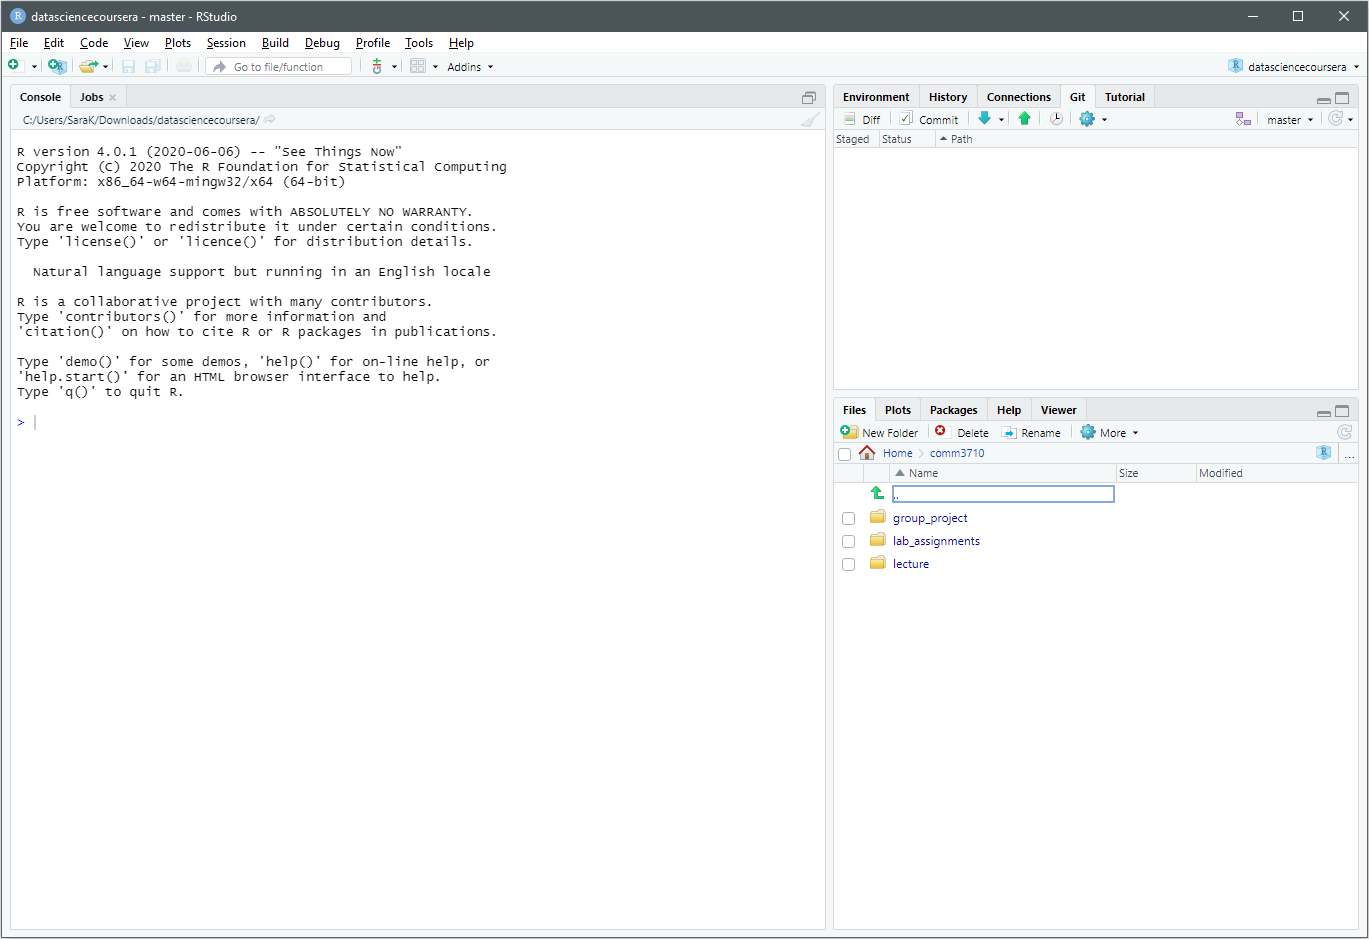
\includegraphics{LA.1_RStudio.png}

\hypertarget{comm-3710-working-directory}{%
\subsubsection{COMM 3710 working
directory}\label{comm-3710-working-directory}}

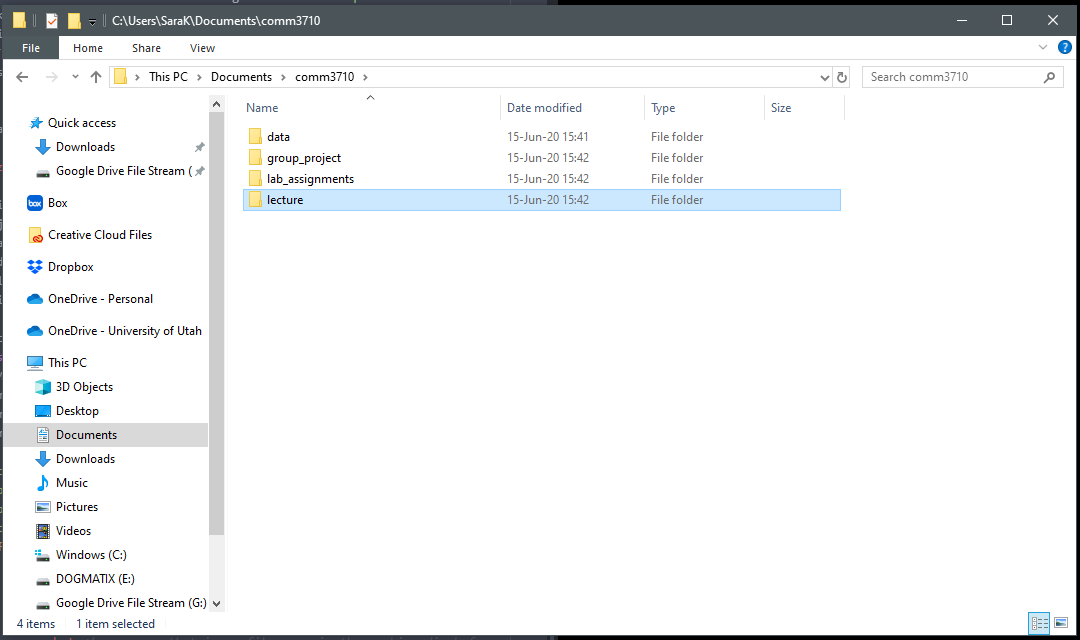
\includegraphics{LA.1_workingdir.png}

\hypertarget{part-ii}{%
\section{Part II}\label{part-ii}}

Read the \href{https://rpubs.com/yesun/Comm3710_helpwithR}{R help guide}
(especially Sections 2.1 - 2.3). Then, follow these following steps to
answer the question.

\begin{enumerate}
\def\labelenumi{\arabic{enumi}.}
\item
  Create an object that represents the outcome of \texttt{2\ x\ 5}, and
  assign a name of your choice to this object.\\
\item
  Create a second object that represents the outcome of
  \texttt{45\ -\ 5}, and assign a name of your choice to this object.
\item
  Create a third object that represents the \emph{product} of the first
  two objects, and assign a name of your choice to this object.
\item
  Answer the following question: What is the value of the third object?
\end{enumerate}

\textbf{Submit a screenshot of the R commands that you used to arrive at
your answer to Question 4. This screenshot should include all three
objects from Questions 1-3 and the answer to Question 4.}

\end{document}
